\documentclass[11pt]{article}
\usepackage{amsmath}
%\usepackage{extsizes}
\usepackage{amsmath,amssymb}
%\usepackage{omegavn,ocmrvn}
%\usepackage[utf8x]{inputenc}
\usepackage[utf8]{vietnam}

\usepackage{listings}
\lstset{language=Python}          % Set your language (you can change the language for each code-block optionally)
	

\usepackage{longtable}
\usepackage{answers}
\usepackage{graphicx}
\usepackage{array}
\usepackage{pifont}
\usepackage{picinpar}
\usepackage{enumerate}
\usepackage[top=3.0cm, bottom=3.5cm, left=3.5cm, right=2.5cm] {geometry}
\usepackage{hyperref}


\newtheorem{bt}{Câu}
\newcommand{\RR}{\mathbb R}
\Newassociation{sol}{Solution}{ans}
\newtheorem{ex}{Câu}
\renewcommand{\solutionstyle}[1]{\textbf{ #1}.}


\begin{document}
% \noindent
\begin{tabular*}
	{\linewidth}{c>{\centering\hspace{0pt}} p{.7\textwidth}}
	Trường ĐHKHTN, ĐHQGHN & {\bf Học Kỳ 1 (2021-2022)}
	\tabularnewline
	K64 TTƯD - Thầy Hà Phi & {\bf Bài Tập Giải Tích Số. No 3a \\ Phương pháp phân đôi  \\ \today}
	% Exercises on pages 239, 240 Cheney/Kincaid are really nice
	\tabularnewline
	\rule{1in}{1pt}  \small  & \rule{2in}{1pt} %(Due date:)
	\tabularnewline
	
	%  \tabularnewline
	%  &(Đề thi có 1 trang)
\end{tabular*}
%
% \Opensolutionfil{ans}[ans1]

\begin{bt}
Hãy viết hàm phân đôi (bisection trong Python có dạng) sau:
%
\begin{lstlisting}[frame=single] 
def bisection(f,a,b,nmax,tol):
    return c, err, n
\end{lstlisting}
%
trong đó f là hàm số; a,b: là điểm đầu và điểm cuối của đoạn ta tìm nghiệm; nmax: số lượng tối đa các phép lặp; tol: sai số nhỏ nhất cho phép; c: nghiệm xấp xỉ;
err: đánh giá cận trên của sai số tuyệt đối của nghiệm xấp xỉ; n: số bước lặp thực hiện để tìm c.\\
\textbf{Trong các câu sau hãy sử dụng chính hàm bisection vừa viết trong câu 1 để thực hành trong Python.}
\end{bt}

\begin{bt} 
Sử dụng phương pháp phân đôi để tìm nghiệm của các phương trình sau, với sai số $tol=1e-9$.\\ 
(a) Các nghiệm thực của phương trình $x^3 - x^2 - x + 1 = 0$. \\
(b) Nghiệm của phương trình $x^2 = 1 + 0.3\ \cos(x)$. \\
(c) Nghiệm dương nhỏ nhất của $cos(x) = 1/2 + sin (x)$. \\
(d) Nghiệm của $x = e^{-x}$. \\
(e) Nghiệm dương nhỏ nhất của phương trình $e^{-x} = sin(x)$. 
\end{bt}

\begin{bt}
	Vẽ đồ thị của hai hàm số ở 2 vế của phương trình $x = tan(x)$, và quan sát giao điểm của 2 đồ thị đó.\\
	(a) Dựa vào đồ thị, hãy chọn 2 điểm đầu mút $a$, $b$ cho phương pháp phân đôi để tìm nghiệm dương nhỏ nhất của phương trình $x = tan (x)$, với độ chính xác 
	$\epsilon=1e-9$. \\
	(b) Tìm nghiệm gần $100$ nhất của phương trình $x = tan(x)$ sử dụng phương pháp phân đôi.
\end{bt}

\begin{bt}
a) Viết script trong Python sử dụng phương pháp phân đôi để tìm tất cả các nghiệm của phương trình sau với độ chính xác $\epsilon=1e-6$.
\[ f(x) := 32x^6 - 48x^4 +18x^2 - 1 = 0.  \] 
b) Tính số bước lặp theo công thức trong lý thuyết và so sánh với kết quả lập trình trong Python.
\end{bt}

\begin{bt} % Exercise 7, page 78, Atkinson/Han
a) Sử dụng phương pháp phân đôi để giải phương trình sau với độ chính xác $\epsilon=1e-6$. 
%
\[ f(x) := x^3-3x^2+3x-1 = 0. \]
%
Hãy thử nghiệm 3 phương pháp khác nhau để gọi giá trị của hàm $f$: 1) dùng dạng đã cho 2) đảo ngược thứ tự 3) dùng dạng đa thức trong lược đồ Horner $f(x) = -1+x(3+x(-3+x))$. \\
b) Chọn 1 trong 3 phương pháp trên và thử các đoạn $[a,b]$ khác nhau, ví dụ, $[0, 1.5]$, $[0.5, 2.0]$, và $[0.5, 1.1]$. Giải thích sự khác nhau trong các kết quả thu được. 
\end{bt}

\centerline{-----------Hết-----------}

%\vspace{1cm}
%\noindent{\bf Chú ý:} {\it Cán bộ coi thi không giải thích gì thêm}\\
%\vspace{0.4cm}
%\noindent{\bf Họ và tên học sinh: \rule{3in}{.01pt} Lớp: \hrulefill}
%\Closesolutionfile{ans}
%\newpage
%\begin{center}
%{\LARGE{\bf ĐÁP ÁN}}
%\end{center}
%\begin{Solution}{1}
	\begin{figure}[h!]
		\centering
		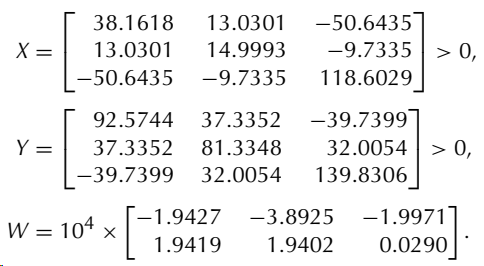
\includegraphics[width=0.7\linewidth]{Solution1/screenshot001}
		\caption[Exercise 1.2.5, Burden-Faires, 8ed.]{}
		\caption{}
		\label{fig:screenshot001}
	\end{figure}
\end{Solution}
 
   
\end{document}